
\begin{itemize}
\item How to convert files in batch 

\begin{verbatim}
> convert '*.png' converted_%04d.jpg
\end{verbatim}

\item How to Remove unwanted empty lines in a file with vi(m)\\
Use either of the following commands to delete all empty lines: 
\begin{verbatim}
:g/^$/d
:v/./d
\end{verbatim}
If you want to delete all lines that are empty or that contain only whitespace 
characters (spaces, tabs), use either of: 
\begin{verbatim}
:g/^\s*$/d
:v/\S/d
\end{verbatim}

\item How to find LAPACK
\begin{verbatim}
## BLAS: /usr/lib/x86_64-linux-gnu/blas/libblas.so.3.7.1
## LAPACK: /usr/lib/x86_64-linux-gnu/lapack/liblapack.so.3.7.1
\end{verbatim}

\item How to apt-get MUMPS

\begin{verbatim}
> sudo apt-get install libmumps-seq-dev
\end{verbatim}

\item How to remove a big file wrongly committed

\begin{verbatim}
> git filter-branch --tree-filter 'rm -rf path/to/your/file' HEAD
> git push
\end{verbatim}

\item How to check your disk usage (ubuntu)\\

Disk Usage Analyzer (aka Baobab) is a graphical, menu-driven viewer 
that you can use to view and monitor your disk usage and folder structure. 
It is part of every GNOME desktop.

\begin{verbatim}
> baobab
\end{verbatim}

\begin{center}
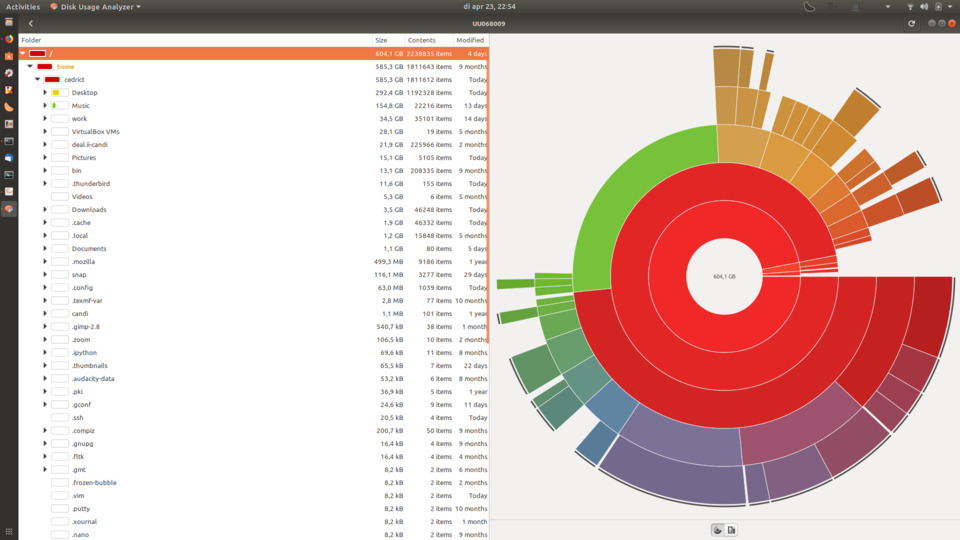
\includegraphics[width=7cm]{images/baobab}
\end{center}


\item How to convert images into another format in the command line

\begin{verbatim}
> convert file.png file.jpg
\end{verbatim}

You can also resize on the fly:

\begin{verbatim}
> convert -resize 70% file.png file.jpg
\end{verbatim}



\end{itemize}

